% !TEX root = ../../../main.tex
% !TEX encoding = UTF-8 Unicode
% !TEX encoding = UTF-8

\section{Kostenarten - KL}
% \textit{Autor: Klaus Landsdorf}

\label{section_kostenarten}
Kalkulationen benötigen bestimmte eindeutige Kostenarten, die in einem Kostenartenplan aufgestellt und in einer Kostenartenrechnung kontrolliert werden können. Die eindeutigen Kostenarten können in Kostenartenkategorien bzw. Kostenartengruppen zusammenfließen. Im folgenden soll festgehalten werden, was man für eine Kalkulation und deren Kontrolle w\"ahrend der Umsetzung bedenken sollte.

\begin{figure}[h!]
	\centering
	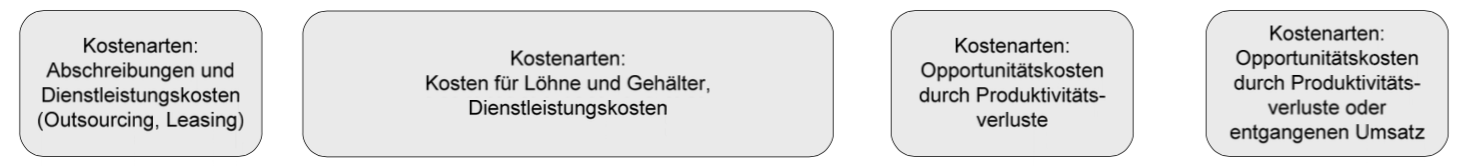
\includegraphics[width=\textwidth]{kapitel/gruppe4_2/bilder/beispiel_kostenarten_TCO}
	\caption{Beispiel von Kostenarten in der TCO-Methode}
	\label{fig_kostenarten_TCO}
\end{figure}

Die Kostenarten der Abbildung \ref{fig_kostenarten_TCO} nach Hansen\footnote{\autocite[495]{hansen_business_2009}, \autocite[Vgl.][314, 355]{muller2013betriebswirtschaftslehre}} finden sich in der von Krcmar benannten TCO-Methode - \enquote{Total Cost of Ownership} - wieder. Aus den bewerteten Daten der Kostenarten können periodische Durchschnittswerte ermittelt werden, aus denen dann für die Zukunft neue Abschätzungen gewonnen werden.

\clearpage

In einer ABC-Analyse kann eine weitere Klassifizierung vorgenommen werden, um aufzuzeigen welche Kostenarten auf jeden Fall (A-Klasse) anfallen, welche im besten Fall noch erledigt werden sollen (B-Klasse) und welche man optional (C-Klasse) aufwenden sollte.

Die Kostenarten in der Tabelle \ref{tab_gliederung_kostenarten} sind die erweiterten Grundelemente der Abbildung \ref{fig_kostenarten_TCO} zur Wertsteigerung durch Wertschöpfung\footnote{\autocite[125-128]{reim_erfolgsrechnung_2015}}, die laut Reim in die Kostenartenrechnung fließen sollten. Die Tabelle \ref{tab_gliederung_kostenarten}\footnote{\autocite[138]{reim_erfolgsrechnung_2015}} soll, m\"oglichen Projekten des integrierten Informationsmanagements der Hochschule Emden/Leer, als wiederverwendbare Übersicht dienen, damit in den notwendigen Kalkulationen alle Kosten erfasst werden. Warum Kostenarten so interessant sind, hat Reim in einem kurzen Satz zusammengefasst: „Die Kostenartenrechnung erfasst, systematisiert und periodisiert die Kosten.“\footnote{\autocite[137-147]{reim_erfolgsrechnung_2015}} 

\begin{table}[h!]
\begin{tabularx}{\textwidth}{|X|X|}
	\hline \textbf{Gliederungsmerkmale nach} & \textbf{Kostenartengruppen} \\ 
	\hline der Art der verbrauchten Einsatzgüter & \begin{itemize}
		\item Materialkosten
		\item Personalkosten
		\item Fremdleistungskosten
		\item Kalkulatorische Kosten
	\end{itemize} \\ 
	\hline der Herkunft der verbrauchten Einsatzgüter & \begin{itemize}
		\item Primäre Kosten
		\item Sekundäre Kosten	
	\end{itemize}  \\ 
	\hline der Beschäftigungsabhängigkeit & \begin{itemize}
		\item Variable Kosten
		\item Fixe Kosten
	\end{itemize} \\ 
	\hline der Art der Verrechnung & \begin{itemize}
		\item Einzelkosten
		\item Gemeinkosten
		\item Sondereinzelkosten
	\end{itemize} \\ 
	\hline 
\end{tabularx}
	\caption{Kostenarten der Gesamtkosten in mögliche Gliederungsmerkmale gruppiert}
	\label{tab_gliederung_kostenarten}
\end{table}

Ein systematischer und periodischer Blick auf die Gesamtkosten, nach den verschiedenen Gliederungsmerkmalen der Tabelle \ref{tab_gliederung_kostenarten}, wird f\"ur die Planung und sp\"atere Kontrolle der ben\"otigten Mittel eine passende Hilfe f\"ur den CIO sein. Für die Wertschöpfung ist das Gliederungsmerkmal nach Art der verbrauchten Einsatzgüter zu betrachten.

\subsection{Kostenarten in Hochschulen}
Im Hochschulbereich betrachtet man besonders die Kostenarten der Einzelkosten und Gemeinkosten. Die Kostenarten müssen, im universitären Umfeld, besonders in Forschungsprojekten mit Drittmitteln genau aufgeschlüsselt und zugewiesen werden, um einen transparenten Überblick zu erhalten, wo die Kosten anfallen und wo die Drittmittel hinfließen.\footnote{\cite{pkl_2005}}

Die genaue Form der Kostenerfassung sollte in diesem Projekt angewendet werden. Es sollte eine sekundäre Kostenart Informationsmanagement geben, damit die Kosten zugeordnet und überwacht werden können. Daraus können folgende Projekte im Vorfeld besser eingeschätzt werden. Dies wird durch die Einzelkosten erreicht, wohingegen die Gemeinkosten in mehreren Bereichen der Hochschule anfallen und der Aufwand einer Einzelzuordnung nicht vertretbar oder zielführend ist.

Die kalkulatorischen Kosten teilen sich in die Zusatzkosten und die Anderskosten und sind in der Abbildung \ref{fig_abgrenzung_aufwand} tabellarisch eingeordnet. Anderskosten sind Kostenarten die noch nicht benannt sind bzw. erkannt werden, aber nicht in der laufenden Periode zugeordnet werden können. 

\begin{figure}[h!]
	\centering
	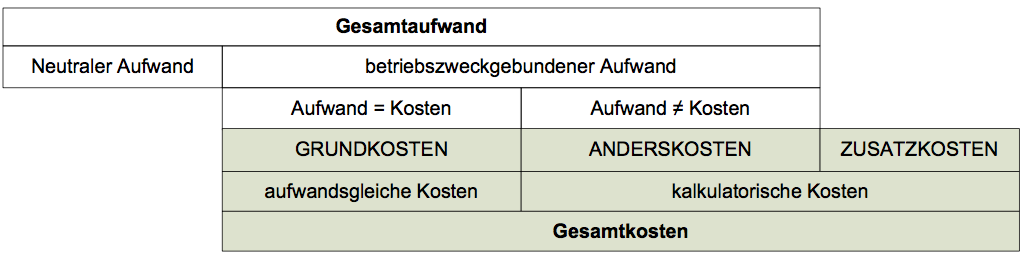
\includegraphics[width=\textwidth]
	{kapitel/gruppe4_2/bilder/abgrenzung_aufwand}
	\caption{Abgrenzung Aufwand - Kosten, nach Handbuch der Kostenartenrechnung 2005}
	\label{fig_abgrenzung_aufwand}
\end{figure}

In der Betrachtung der primären und sekundären Kostenarten, sind in einer Hochschule die sekundären Kostenarten besonders interessant, da sie die Kosten der Bereiche zusammenfassen und einen Überblick verschaffen.

Wie das Beispiel der Abbildung \ref{fig_uebergang_primaerkosten} zeigt, bauen sich die sekundären Kosten, in der Kostenstellenrechung, durch das Zusammenfließen der primären Kosten auf. An der Leibnitz Universität Hannover (LUH) wurden, für das SAP-System, 900 Primärkostenarten in 140 Sekundärkostenarten verdichtet und zugeordnet.\footnote{\cite{pkl_2005}}

\begin{figure}[h!]
	\centering
	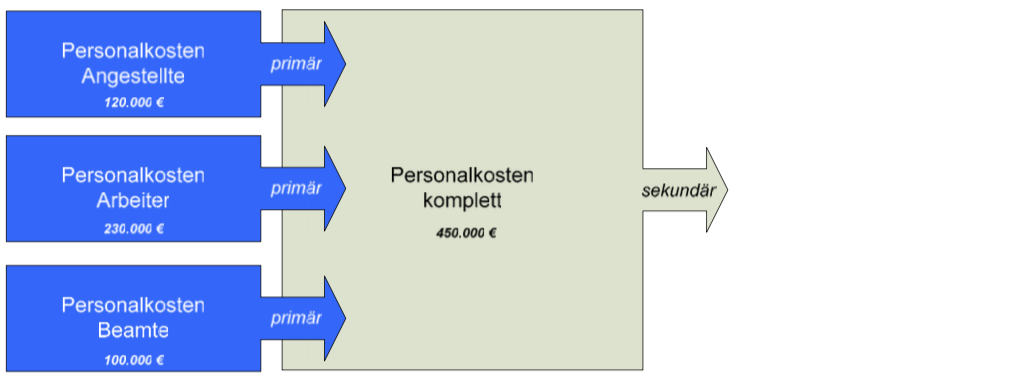
\includegraphics[width=\textwidth]
	{kapitel/gruppe4_2/bilder/uebergang_primaerkosten}
	\caption{Übergang von Primär- in Sekundärkosten,\\nach Handbuch der Kostenartenrechnung 2005}
	\label{fig_uebergang_primaerkosten}
\end{figure}

Diese Primärkostenarten und Sekundärkostenarten sind im Jahr 2005 im Rahmen des Projektes “Uni2001” für ganz Niedersachsen abgestimmt worden und im SAP-System eingepflegt. Ein entsprechender Abgleich mit Mitarbeitern der Hochschule Emden/Leer für die vorhandenen und besonders der genutzten Kostenarten sollte bei der konkreten Projektplanung unbedingt erfolgen. Die Hierarchie der Kostenarten der Hochschule sollten sich ähnlich, wenn nicht sogar gleich, dem Beispiel der Abbildung \ref{fig_kostenartenhierarchie_uni2001} der LUH darstellen.

\begin{figure}[h!]
	\centering
	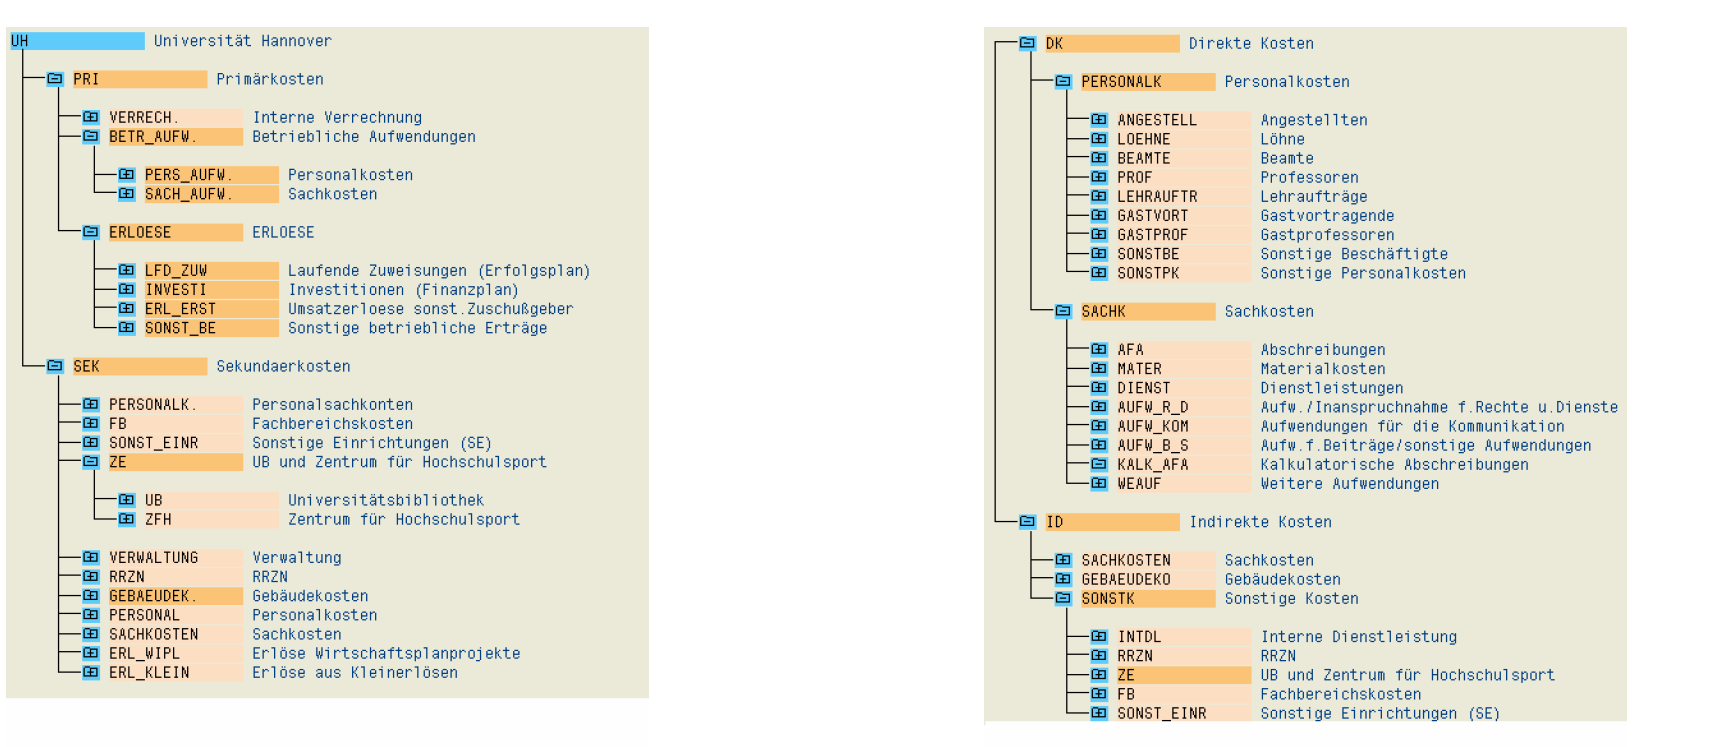
\includegraphics[width=\textwidth]
	{kapitel/gruppe4_2/bilder/kostenartenhierarchie_uni2001}
	\caption{Kostenartenhierarchie der Hochschulen Uni2001,\\nach Handbuch der Kostenartenrechnung 2005}
	\label{fig_kostenartenhierarchie_uni2001}
\end{figure}

% !TEX root = ../../../main.tex
% !TEX encoding = UTF-8 Unicode
% !TEX encoding = UTF-8

\subsection{Kostenarten in der IT}
In einer Hochschule ist ein Rechenzentrum für die Aufgaben der IT zuständig.
Der Rechenzentrumsleiter ist in einem Netzwerk, aus leitenden Personen der Hochschule, das Zentrum der personellen IT-Komponenten. In der IT einer Hochschule werden direkte Kosten zwischen den Primärkategorien Hard- und Software, operativer Betrieb und Verwaltung differenziert.\footnote{\autocite[494]{hansen_business_2009}}

Zusätzlich ist ein Rechenzentrum der Hochschule, nach Interview-Aussage des Rechenzentrumsleiters der Hochschule Emden/Leer, jährlich auf ein bestimmtes Budget festgelegt. Danach ist die Tabelle \ref{tab_auswahl_IT_kostenarten}\footnote{\autocite[493-498]{hansen_business_2009}} zu beachten, welche Kosten budgetiert sind und welche nicht. Die folgenden Tabellen sind für den Rechenzentrumsleiter als Kontrollhilfe angedacht, damit keine IT-Kostenarten unbeachtet bleiben.

\begin{table}[h!]
	\begin{tabularx}{\textwidth}{|X|X|}
		% Überschriften
		\hline \textbf{Budgetierte Kosten}  &  \textbf{Nicht budgetierte Kosten}\\
		% Zeile 1
		\hline Software-Entwicklung 
			\begin{itemize}
				\item Neuentwicklung und Anpassungen
				\item Personal- und Sachkosten	
			\end{itemize}  
		& Negative Produktivitätseffekte
			\begin{itemize}
				\item Antwort-, Rüst- und Bearbeitungszeit
				\item Motivation
				\item Ergonomie
			\end{itemize} \\ 
		% Zeile 2	
		\hline Kommunikation \begin{itemize}
			\item Netzwerk
			\item Personal- und Sachkosten			
		\end{itemize} & Ausfall \begin{itemize}
			\item geplant
			\item ungeplant
		\end{itemize} \\ 
		% Zeile 3
		\hline Hardware / Software \begin{itemize}
			\item Abschreibung, Miete und Leasing
			\item Entsorgung
			\item Client / Server
			\item Administration	
		\end{itemize} & Endbenutzer \begin{itemize}
			\item Peer-Support (selbst/gegenseitig)
			\item Unproduktives Konfigurieren
			\item Qualifizierung (selbst /gegenseitig)
		\end{itemize}  \\
		% Zeile 4
		\hline Support &   \\
		% Zeile 5 
		\hline Systembetrieb und Systemmanagement & \\
		\hline
	\end{tabularx}
	\caption{Auszug der IT-Kostenarten nach Krcmar}
	\label{tab_auswahl_IT_kostenarten}
\end{table}

\clearpage 

Als spezielle IT-Kostenarten werden von Gadatsch und Mayer aufgelistet\footnote{\autocite[349]{gadatsch_masterkurs_2014}}:

\begin{table}[h!]
	\begin{tabularx}{\textwidth}{|l|X|}
		% Überschriften
		\hline \textbf{Sekundäre Kostenarten}  &  \textbf{Primäre Kostenarten}\\
		% Zeile 1
		\hline Hardware-Kosten &
		\begin{itemize}
			\item Miete / Leasing
			\item Hardware
			\item Leitungsgebühren
			\item Wartung
		\end{itemize} \\ 
		% Zeile 2	
		\hline Software-Kosten  & 
		\begin{itemize}
			\item Miete / leasing
			\item Software
			\item eigene Entwicklung
			\item Externe Wartung
			\item Beratung
		\end{itemize} \\ 
	% Zeile 3
	\hline Daten-Kosten &
	\begin{itemize}
		\item Beratung
		\item Kauf
	\end{itemize}  \\
	% Zeile 4
	\hline Sonstige IT-Kosten &
		\begin{itemize}
			\item IT-Verbrauchsmaterial
			\item IT-Versicherungen
			\item Beiträge zu Fachverbänden
			\item IT-Fachliteratur
			\item IT-Schulungen
		\end{itemize}\\
	% Zeile 5 
	\hline Innerbetriebliche IT-Leistungsverrechnung & 
	\begin{itemize}
		\item Umlagen
		\item Entwicklungskosten
		\item Benutzerservice
	\end{itemize}\\
	\hline
\end{tabularx}
\caption{Auflistung der speziellen IT-Kosten, nach Gadatsch \& Mayer}
\label{tab_auflistung_spezielle_IT_Kosten}
\end{table}

Die Kostenarten aus den Auflistungen der Tabellen \ref{tab_auswahl_IT_kostenarten} und \ref{tab_auflistung_spezielle_IT_Kosten} eignen sich laut Hansen\footnote{\autocite[493-498]{hansen_business_2009}} für die Betrachtung der Kosten an einer Hochschule.

Als mögliche Nutzung der Kostenarten, schlägt Krcmar die TCO-Methode als Bewertungstechnik vor, was ausführlicher im Kapitel \ref{kosten_zeit_anwendung} beschrieben und zur Teilkalkulation verwendet wird.\footnote{\autocite[144]{krcmar_einfuhrung_2015}} Die TCO-Methode nutzt die Kostenarten, um die wirtschaftlichen Auswirkungen in der IT aufzuzeigen.

\clearpage

Vor allem im Bezug auf Kostenarten und IT wird als Trend ein IT-Controller empfohlen\footnote{\autocite[49]{gadatsch_masterkurs_2014}}, um eine erfolgreiche Wertschöpfung in der IT zu erreichen. Der IT-Controller hat die Transparenzverantwortung gegenüber dem CIO und entlastet ihn damit, wodurch der CIO sich gezielt auf seine Entscheidungsverantwortung konzentrieren kann.\footnote{\url{http://vfhinf.oncampus.de/loop/Zusammenarbeit_zwischen_CIO_und_IT-Controller}} Sollte die Hochschule Emden/Leer dieser Empfehlung folgen, ist besonders auf die klare Rollenverteilung zwischen CIO und IT-Controller zu achten. Ihre Kompetenzen dürfen sich nur in Ausnahmen gegenseitig blockieren. Der CIO sollte im Zweifel eine Entscheidungsgewalt haben und passend dazu die Konsequenzen alleine tragen, wenn er die Entscheidungsgewalt nutzt. Im idealen Fall tragen Beide die endgültige Entscheidung in einem Kompromiss.

Gerade in einem solch zentralen Projekt, mit hohem Anteil an IT-lastigen Themen, ist es zumindest empfehlenswert über einen IT-Controller nachzudenken.\footnote{\autocite[11-15]{stratmann_it_2013}} Besonders ist hier auch die höhere Komplexität zu beachten, die jeweils in der IT, DFG geförderter Referenzprojekte, entstand. Einige Referenzprojekte werden später im Kapitel \ref{section_projekt_beispiele} vorgestellt und mit der Hochschule Emden/Leer verglichen. Doch zuvor sollen im Kapitel \ref{section_verfahren_schaetzung} ausgewählte Kosten- und Zeitschätzungen erläutert werden, wie die empfohlenen Kostenarten in der Kalkulation Verwendung finden.









